\documentclass[aspectratio=169]{beamer}

\usepackage{iftex}
\providecommand{\dunenoirsetupfonts}{}
\newcommand{\DuneNoirLocalFontPath}{fonts}

\newcommand{\DuneNoirMonoFallback}{%
  \IfFontExistsTF{JetBrainsMono Nerd Font Propo}{
    \setmonofont{JetBrainsMono Nerd Font Propo}[Scale=0.92]
  }{
    \IfFontExistsTF{JetBrainsMono Nerd Font}{
      \setmonofont{JetBrainsMono Nerd Font}[Scale=0.92]
    }{
      \setmonofont{Courier New}[Scale=0.92]
    }
  }
}

\newcommand{\DuneNoirSansFallback}{%
  \IfFontExistsTF{IBM Plex Sans}{
    \setsansfont{IBM Plex Sans}
    \setmainfont{IBM Plex Sans}
  }{
    \IfFontExistsTF{Helvetica Neue}{
      \setsansfont{Helvetica Neue}
      \setmainfont{Helvetica Neue}
    }{
      \setsansfont{Arial}
      \setmainfont{Arial}
    }
  }
}

\newcommand{\DuneNoirUseHelvetica}{%
  \renewcommand{\dunenoirsetupfonts}{%
    \IfFontExistsTF{Helvetica Neue}{
      \setsansfont{Helvetica Neue}
      \setmainfont{Helvetica Neue}
    }{
      \IfFontExistsTF{Helvetica}{
        \setsansfont{Helvetica}
        \setmainfont{Helvetica}
      }{
        \DuneNoirSansFallback
      }
    }
    \DuneNoirMonoFallback
  }%
}

\newcommand{\DuneNoirUseOpenSans}{%
  \renewcommand{\dunenoirsetupfonts}{%
    \IfFileExists{\DuneNoirLocalFontPath/OpenSans.ttf}{
      \setsansfont{Open Sans Custom}[
        Path=\DuneNoirLocalFontPath/,
        UprightFont={OpenSans.ttf},
        ItalicFont={OpenSans-Italic.ttf},
        BoldFont={OpenSans.ttf},
        BoldItalicFont={OpenSans-Italic.ttf},
        BoldFeatures={FakeBold=1.45},
        BoldItalicFeatures={FakeBold=1.45}
      ]
      \setmainfont{Open Sans Custom}[
        Path=\DuneNoirLocalFontPath/,
        UprightFont={OpenSans.ttf},
        ItalicFont={OpenSans-Italic.ttf},
        BoldFont={OpenSans.ttf},
        BoldItalicFont={OpenSans-Italic.ttf},
        BoldFeatures={FakeBold=1.45},
        BoldItalicFeatures={FakeBold=1.45}
      ]
    }{
      \DuneNoirSansFallback
    }
    \DuneNoirMonoFallback
  }%
}

\newcommand{\DuneNoirUseDosis}{%
  \renewcommand{\dunenoirsetupfonts}{%
    \IfFileExists{\DuneNoirLocalFontPath/Dosis.ttf}{
      \setsansfont{Dosis Custom}[
        Path=\DuneNoirLocalFontPath/,
        UprightFont={Dosis.ttf},
        ItalicFont={Dosis.ttf},
        BoldFont={Dosis.ttf},
        BoldItalicFont={Dosis.ttf},
        ItalicFeatures={FakeSlant=0.16},
        BoldFeatures={FakeBold=1.6},
        BoldItalicFeatures={FakeBold=1.6,FakeSlant=0.16}
      ]
      \setmainfont{Dosis Custom}[
        Path=\DuneNoirLocalFontPath/,
        UprightFont={Dosis.ttf},
        ItalicFont={Dosis.ttf},
        BoldFont={Dosis.ttf},
        BoldItalicFont={Dosis.ttf},
        ItalicFeatures={FakeSlant=0.16},
        BoldFeatures={FakeBold=1.6},
        BoldItalicFeatures={FakeBold=1.6,FakeSlant=0.16}
      ]
    }{
      \DuneNoirSansFallback
    }
    \DuneNoirMonoFallback
  }%
}

\newcommand{\DuneNoirUseKoHo}{%
  \renewcommand{\dunenoirsetupfonts}{%
    \IfFileExists{\DuneNoirLocalFontPath/KoHo-Regular.ttf}{
      \setsansfont{KoHo Custom}[
        Path=\DuneNoirLocalFontPath/,
        UprightFont={KoHo-Regular.ttf},
        BoldFont={KoHo-Bold.ttf},
        ItalicFont={KoHo-Italic.ttf},
        BoldItalicFont={KoHo-BoldItalic.ttf}
      ]
      \setmainfont{KoHo Custom}[
        Path=\DuneNoirLocalFontPath/,
        UprightFont={KoHo-Regular.ttf},
        BoldFont={KoHo-Bold.ttf},
        ItalicFont={KoHo-Italic.ttf},
        BoldItalicFont={KoHo-BoldItalic.ttf}
      ]
    }{
      \DuneNoirSansFallback
    }
    \DuneNoirMonoFallback
  }%
}

\DuneNoirUseHelvetica
\makeatletter
\input{../dune_dark_template_lab/beamerthemeDUNENoir.sty}
\makeatother

\ifPDFTeX
  \usepackage[T1]{fontenc}
  \usepackage[utf8]{inputenc}
\fi

\usepackage{amsmath,amssymb,mathtools}
\usepackage{graphicx,booktabs,array,tabularx,hyperref}
\usepackage{siunitx}
\usepackage{appendixnumberbeamer}
\usepackage[dvipsnames]{xcolor}

\DeclareSIUnit{\channel}{channel}
\DeclareSIUnit{\trigger}{trigger}
\DeclareSIUnit{\word}{word}
\DeclareSIUnit{\sample}{sample}
\sisetup{detect-all,per-mode=symbol}

\title[DAPHNE Dead-Time Models and Grouped Hermes]{DAPHNE Dead-Time Models and Grouped Hermes}
\subtitle{Model definitions, full-chain RTL simulation, and current resource status}
\author{Manuel Arroyave}
\date{May 14, 2026}
\newcommand{\mydate}{May 14, 2026}

\newcommand{\fdhdrate}{\SI{4.6}{\kilo\hertz\per\channel}}
\newcommand{\fdhddead}{\SI{7.6}{\percent}}
\newcommand{\builderbusy}{\SI{16.592}{\micro\second}}
\newcommand{\wordshare}{\SI{3.125}{\mega\word\per\second\per\channel}}
\newcommand{\throughputceiling}{\SI{25.6}{\kilo\hertz\per\channel}}
\newcommand{\currentdead}{\SI{7.5}{\percent}}
\newcommand{\shortdead}{\SI{4.2}{\percent}}
\newcommand{\ringzerodead}{\SI{4.2}{\percent}}
\newcommand{\ringfiftydead}{\SI{2.6}{\percent}}
\newcommand{\coalescedgatedead}{\SI{5.2}{\percent}}
\newcommand{\coalescedopendead}{\SI{0.0}{\percent}}
\newcommand{\coalbranch}{\texttt{coal-tail512}}
\newcommand{\coalrtldead}{\SI{4.5}{\percent}}
\newcommand{\coalrtlhigh}{\SI{11.8}{\percent}}
\newcommand{\coalbram}{\num{139}/\num{144}}
\newcommand{\coalluts}{\num{105404}}
\newcommand{\coalwns}{\SI{0.103}{\nano\second}}
\newcommand{\groupbranch}{\texttt{marroyav/grouped-hermes-resource-build-candidate}}
\newcommand{\groupcommit}{\texttt{77682da}}
\newcommand{\groupfivewns}{\SI{0.053}{\nano\second}}
\newcommand{\groupfiveluts}{\num{99560}}
\newcommand{\groupfivebram}{\num{103}/\num{144}}
\newcommand{\grouptenluts}{\num{109271}}
\newcommand{\grouptenbram}{\num{128}/\num{144}}
\newcommand{\grouptenwns}{\SI{-1.105}{\nano\second}}

\begin{document}

\begin{frame}
  \titlepage
\end{frame}

\begin{frame}{Argument}
\footnotesize
\textbf{Observed:} at \fdhdrate, the present self-trigger path loses about \fdhddead\ of generated triggers, or about \SI{350}{\trigger\per\second\per\channel}.

\vspace{0.8em}
\textbf{Mitigation path}
\begin{enumerate}
  \item Shorten the record: reduce per-channel builder occupancy.
  \item Add ring buffering: decouple trigger acceptance from immediate waveform packing.
  \item Decide the output contract: overlap is easy to accept; non-overlap requires coalescing.
\end{enumerate}

\vspace{0.8em}
\textbf{Caution:} coalescing is promising as a non-overlap policy, but the current output-full gate makes it a backpressure problem, not yet an HDL performance result.
\end{frame}

\begin{frame}{Observable And Model Boundary}
\footnotesize
\begin{columns}[T,onlytextwidth]
\column{0.45\textwidth}
\begin{block}{Observable}
\[
D(\lambda)=1-
\frac{N_{\mathrm{accepted}}(\lambda)}
     {N_{\mathrm{generated}}(\lambda)}
\]
Accepted means the trigger passed the channel-local rule. It may still wait in the readout path.
\end{block}

\column{0.51\textwidth}
\begin{block}{Simulation layers}
\begin{itemize}
  \item C++ model: fast stochastic ranking of frame policies.
  \item RTL wrapper: live builders and muxes under synthetic triggers.
  \item Hermes chain: real \texttt{tx\_mux} ready/backpressure path.
  \item FPGA build: resource, routing, and timing feasibility.
\end{itemize}
\end{block}
\end{columns}

\end{frame}

\begin{frame}{Model Definitions I: Fixed Records And Rings}
\scriptsize
\begin{tabularx}{\linewidth}{@{}>{\bfseries}p{0.21\linewidth}X@{}}
\toprule
Model & Meaning in this deck \\
\midrule
Legacy 1024 & Old fixed waveform model. One trigger emits a \num{1024}-sample record, modeled as a long per-channel busy interval and \num{232} output words. \\
512 waveform & Same fixed-record contract, but a \num{512}-sample record and \num{120} output words. This is the first-order dead-time reduction. \\
Ring0 & Per-channel \num{2048}-sample ring plus descriptor queue. Trigger acceptance is decoupled from immediate waveform packing, but same-channel spacing is still one full frame. \\
Ring50 & Ring model with relaxed same-channel spacing. For \num{512}-sample records, \texttt{signal\_delay\_steps=16} allows about \num{256} samples of overlap. \\
1024 ring max & Same idea for \num{1024} in the C++ model. The existing 5-bit delay control maxes at \texttt{31}, so the largest tested overlap is \num{496} samples, not exactly \num{512}. \\
\bottomrule
\end{tabularx}

\vspace{0.6em}
\textbf{Important:} accepting overlapping triggers and emitting non-overlapping waveforms are different requirements.
\end{frame}

\begin{frame}{Model Definitions II: Coalesced And Tail}
\scriptsize
\begin{tabularx}{\linewidth}{@{}>{\bfseries}p{0.23\linewidth}X@{}}
\toprule
Model & Meaning in this deck \\
\midrule
Coalesced, current gate & C++ variable-interval model. Nearby trigger windows merge into one emitted physical interval, but the old output-full gate is still applied. \\
Coalesced, relaxed gate & Same C++ interval model with the output gate opened. This is an upper-bound study, not current RTL. \\
\coalbranch & RTL fixed-fragment continuation model. It preserves non-overlap at Ethernet by chaining \num{512}-sample fragments, but it is not true variable-length coalescing. \\
\bottomrule
\end{tabularx}

\vspace{0.8em}
\begin{block}{Boundary}
Coalescing changes the unit of output. It is not only a trigger-acceptance rule; it also changes packet assembly and metadata ownership.
\end{block}
\end{frame}

\begin{frame}{Model Definitions III: Grouped Hermes}
\scriptsize
\begin{tabularx}{\linewidth}{@{}>{\bfseries}p{0.23\linewidth}X@{}}
\toprule
Model & Meaning in this deck \\
\midrule
Grouped+Hermes 5x8 & Full-chain RTL wrapper: \num{40} live \texttt{stc3\_frame\_source} channels, \num{5} serializers, \num{8} channels per serializer, real Hermes \texttt{tx\_mux}, \texttt{READY\_AWARE} enabled, \num{2048}-word Hermes input buffers. \\
Grouped+Hermes 10x4 & Same full-chain RTL wrapper, but \num{10} Hermes sources with \num{4} channels each. It reduces serializer contention in simulation but costs more BRAM/routing in FPGA implementation. \\
\bottomrule
\end{tabularx}

\vspace{0.5em}
\textbf{Current RTL note:} the live grouped-Hermes branch is \num{512}-sample based. The \num{1024} comparison is C++ only unless the RTL constants are parameterized and rebuilt for \num{1024}.
\end{frame}

\begin{frame}{Current Workflow}
\begin{columns}[T,onlytextwidth]
\column{0.62\textwidth}
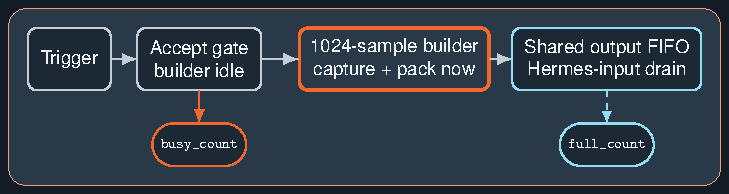
\includegraphics[width=\linewidth,height=0.62\textheight,keepaspectratio]{figures/deadtime_bottleneck_legacy.pdf}

\column{0.34\textwidth}
\small
\begin{block}{Where loss starts}
\[
B=1037\ \mathrm{clocks}
\]
\[
\tau_b=\builderbusy
\]
A second same-channel trigger during this interval increments \texttt{busy\_count}.
\end{block}
\end{columns}
\end{frame}

\begin{frame}{Baseline Data}
\centering
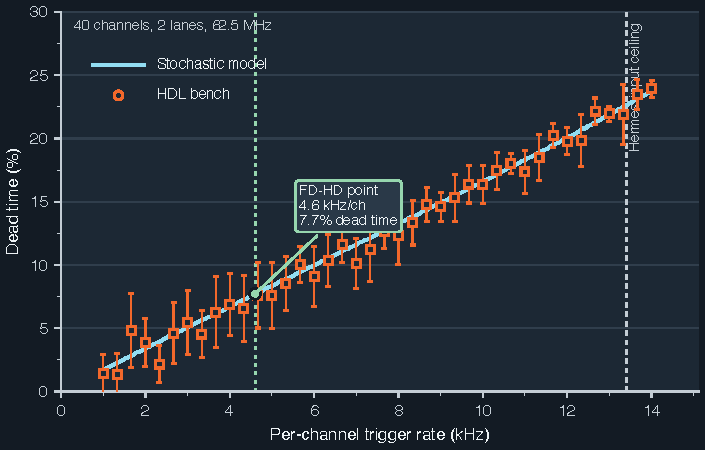
\includegraphics[width=\linewidth,height=0.61\textheight,keepaspectratio]{figures/deadtime_vs_rate_dunenoir_40pt_r8.pdf}

\vspace{0.1em}
\scriptsize\textcolor{noirmuted}{The FD-HD point is already on the rising part of the firmware dead-time curve.}
\end{frame}

\begin{frame}{Study Workflow}
\footnotesize
\begin{enumerate}
  \item Establish the real firmware baseline from successful builds and routed reports on K26.
  \item Use the C++ dead-time model to rank architecture ideas over the full rate range quickly.
  \item Wrap the live RTL in the mezzanine dead-time bench to test the current branch, not a behavioral copy.
  \item Use synth/impl only on the narrowed HDL candidates that survive the C++ and RTL filters.
\end{enumerate}

\vspace{0.6em}
\begin{block}{Why this matters}
The expensive step is implementation on the Kria PL. The workflow is designed to spend iteration time first on model ranking, then on RTL behavior, and only then on place-and-route.
\end{block}
\end{frame}

\begin{frame}{Why This Became A Rabbit Hole}
\small
\begin{enumerate}
  \item \textbf{Shorter fixed records:} \texttt{1024} \(\rightarrow\) \texttt{512}. This helps first and keeps the old output contract.
  \item \textbf{Ring with relaxed spacing:} \texttt{ring50} accepts more triggers, but it does so by allowing overlapping waveform records.
  \item \textbf{Non-overlap redesign:} once overlap is forbidden, the problem moves from trigger acceptance into the frame builder and output seam.
\end{enumerate}

\vspace{0.45em}
\begin{alertblock}{Why this became confusing}
Dead-time mitigation and waveform-contract preservation are not the same problem. The moment overlap is forbidden, trigger acceptance is no longer the whole story: the frame builder and output seam become the real bottleneck.
\end{alertblock}
\end{frame}

\begin{frame}[plain]
\centering
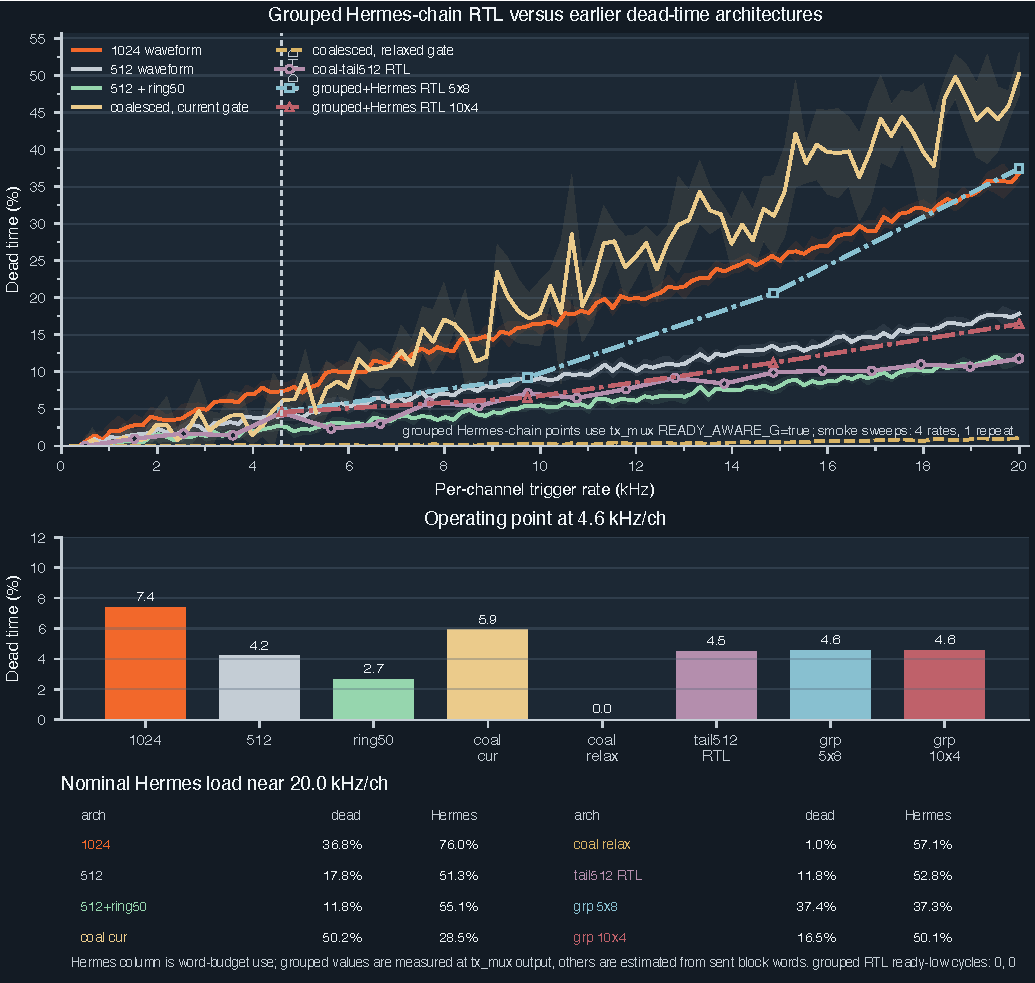
\includegraphics[width=0.98\paperwidth,height=0.96\paperheight,keepaspectratio]{figures/deadtime_grouped_current_arch_compare.pdf}
\end{frame}

\begin{frame}{Latest Full-Chain RTL Points}
\scriptsize
\centering
\begin{tabular}{@{}lrrrrr@{}}
\toprule
Architecture & Sources & Ch/source & \SI{4.6}{\kilo\hertz} & \SI{9.733}{\kilo\hertz} & \SI{20}{\kilo\hertz} \\
\midrule
Grouped+Hermes 5x8 & 5 & 8 & \SI{4.6}{\percent} & \SI{9.2}{\percent} & \SI{37.4}{\percent} \\
Grouped+Hermes 10x4 & 10 & 4 & \SI{4.6}{\percent} & \SI{6.5}{\percent} & \SI{16.5}{\percent} \\
\bottomrule
\end{tabular}

\vspace{0.8em}
\begin{tabular}{@{}lrrrr@{}}
\toprule
Architecture & Hermes load at \SI{4.6}{\kilo\hertz} & \SI{9.733}{\kilo\hertz} & \SI{14.867}{\kilo\hertz} & \SI{20}{\kilo\hertz} \\
\midrule
Grouped+Hermes 5x8 & \SI{13.7}{\percent} & \SI{27.6}{\percent} & \SI{36.5}{\percent} & \SI{37.3}{\percent} \\
Grouped+Hermes 10x4 & \SI{13.7}{\percent} & \SI{28.5}{\percent} & \SI{40.9}{\percent} & \SI{50.1}{\percent} \\
\bottomrule
\end{tabular}

\vspace{0.7em}
\textcolor{noirmuted}{Both RTL sweeps used the real Hermes \texttt{tx\_mux} ready path with no artificial Ethernet or UDP stalls. Source ready-low cycles were zero in these nominal runs.}
\end{frame}

\begin{frame}[plain]
\centering
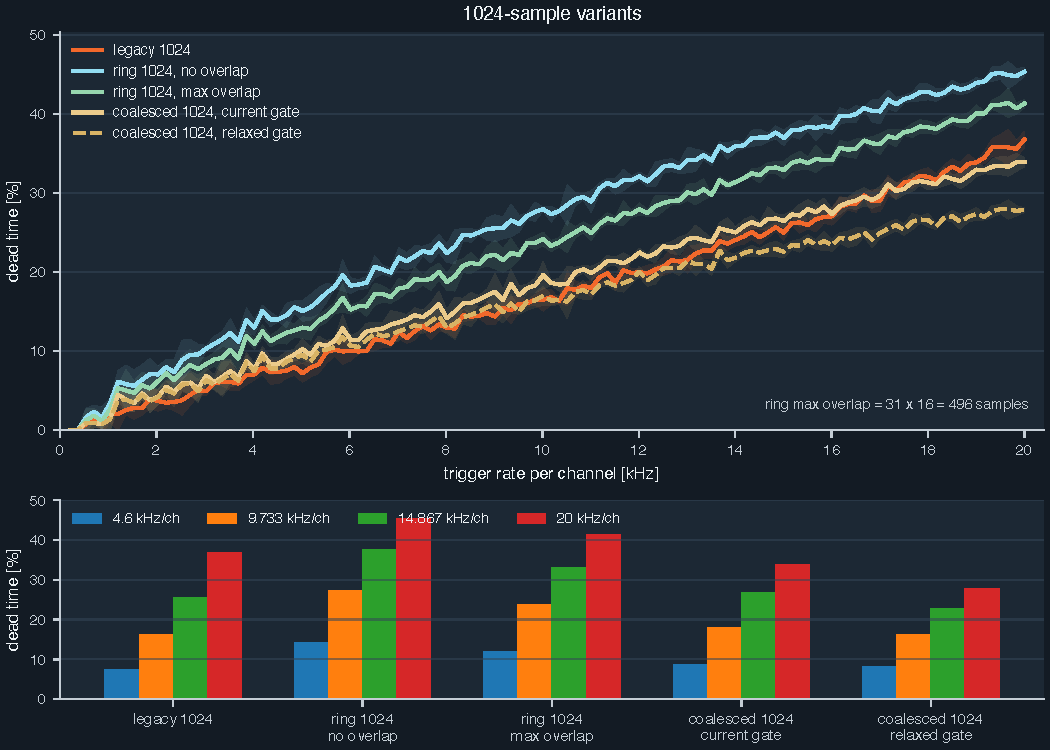
\includegraphics[width=0.98\paperwidth,height=0.96\paperheight,keepaspectratio]{figures/deadtime_1024_variant_compare.pdf}
\end{frame}

\begin{frame}{Methodology Stack}
\footnotesize
\begin{columns}[T,onlytextwidth]
\column{0.32\textwidth}
\begin{block}{C++ model}
\begin{itemize}
  \item fast dense sweeps
  \item architecture ranking
  \item reject-cause accounting
  \item transport sensitivity studies
\end{itemize}
\end{block}

\column{0.32\textwidth}
\begin{block}{RTL wrapper}
\begin{itemize}
  \item live builder + mux
  \item exact branch interface
  \item full-spectrum dead-time sweep
  \item catches contract mistakes
\end{itemize}
\end{block}

\column{0.32\textwidth}
\begin{block}{Implementation}
\begin{itemize}
  \item K26 resource fit
  \item timing closure
  \item packaging path
  \item real feasibility filter
\end{itemize}
\end{block}
\end{columns}

\vspace{0.5em}
\textbf{Discipline:} C++ ranks ideas, RTL validates branch behavior, implementation decides whether the idea survives on hardware.
\end{frame}

\begin{frame}{Why Ring50 Helps}
\centering
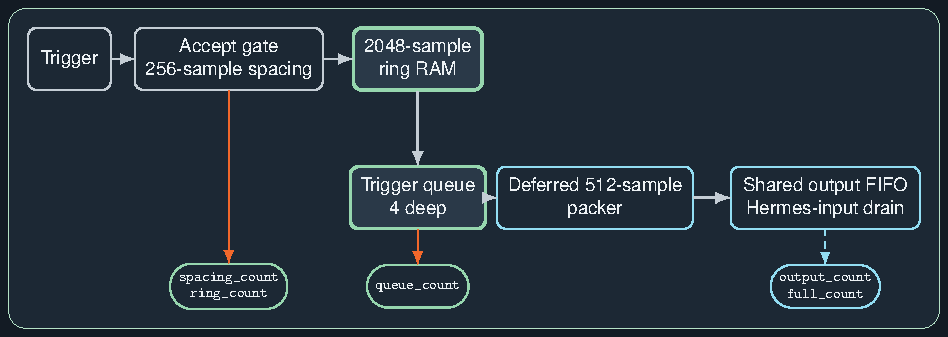
\includegraphics[width=\linewidth,height=0.49\textheight,keepaspectratio]{figures/deadtime_bottleneck_ring2k_overlap.pdf}

\vspace{0.35em}
\footnotesize
\textbf{Mechanism:} trigger metadata waits while samples remain in RAM; the half-frame spacing rule accepts closer triggers.

\textbf{Consequence:} output records can overlap in waveform time.
\end{frame}

\begin{frame}{Why Coalesced Can Work}
\footnotesize
\centering
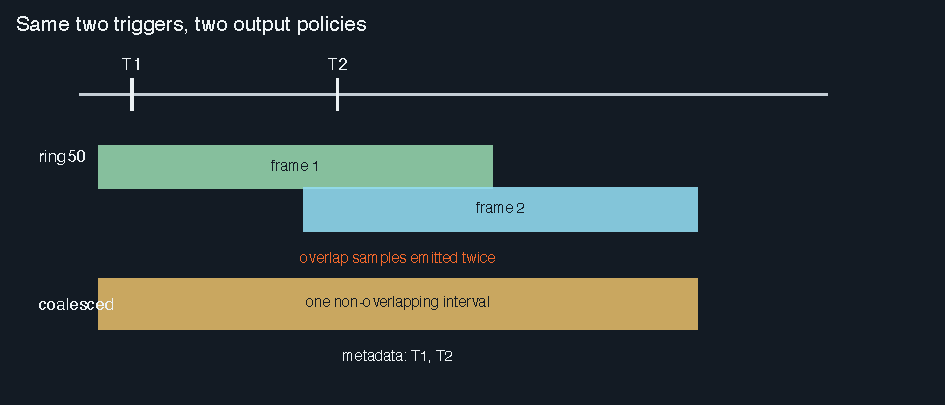
\includegraphics[width=\linewidth,height=0.39\textheight,keepaspectratio]{figures/deadtime_coalescing_timeline.pdf}

\vspace{0.3em}
\begin{itemize}
  \item \texttt{ring50} accepts more by emitting several fixed records, even if they cover the same physical waveform.
  \item \texttt{coalesced} accepts more without overlap because nearby triggers share one emitted waveform interval.
  \item That reduces duplicate waveform words, but only if the assembler and output contract also change.
\end{itemize}
\end{frame}

\begin{frame}{What We Tested: \coalbranch}
\scriptsize
\begin{columns}[T,onlytextwidth]
\column{0.52\textwidth}
\textbf{Policy}
\begin{itemize}
  \item \num{2048}-sample ring per channel
  \item queue depth \num{4}
  \item fixed \num{512}-sample records
  \item no Ethernet-visible overlap
  \item chained continuation when the frame end is still active
\end{itemize}

\column{0.44\textwidth}
\textbf{HDL seam cleanup}
\begin{itemize}
  \item acceptance no longer uses inherited \texttt{prog\_empty/prog\_full}
  \item builder/readout seam is explicit
  \item packet availability is tracked as count
  \item continuation and trigger offset are explicit
\end{itemize}
\end{columns}

\vspace{0.4em}
\textbf{Boundary:} this is still fixed-record transport, not a variable-length coalescer.
\end{frame}

\begin{frame}{Why \coalbranch{} Is Different From Coalesced}
\scriptsize
\begin{columns}[T,onlytextwidth]
\column{0.48\textwidth}
\textbf{\coalbranch}
\begin{itemize}
  \item fixed \num{512}-sample fragments
  \item no overlap visible on Ethernet
  \item if the waveform is still active, open another fixed fragment
\end{itemize}

\column{0.48\textwidth}
\textbf{Coalesced}
\begin{itemize}
  \item one variable-length waveform interval
  \item no overlap visible on Ethernet
  \item nearby triggers extend or merge the same interval
\end{itemize}
\end{columns}

\vspace{0.45em}
\begin{exampleblock}{Practical difference}
\coalbranch\ keeps the fixed record size and fixes the seam. Coalesced changes the unit of output from ``one fixed fragment'' to ``one physical interval''.
\end{exampleblock}
\end{frame}

\begin{frame}{Build And Routing Status}
\scriptsize
\centering
\begin{tabular}{@{}lrr@{}}
\toprule
Metric & 5-source legal route & 10-source illegal route \\
\midrule
CLB LUTs & \groupfiveluts\ (\SI{85.0}{\percent}) & \grouptenluts\ (\SI{93.3}{\percent}) \\
Registers & \num{165056}\ (\SI{70.5}{\percent}) & \num{177485}\ (\SI{75.8}{\percent}) \\
BRAM tiles & \groupfivebram\ (\SI{71.5}{\percent}) & \grouptenbram\ (\SI{88.9}{\percent}) \\
Bitstream & yes & no, route illegal \\
\bottomrule
\end{tabular}

\vspace{0.8em}
\raggedright
\begin{itemize}
  \item 5-source branch: \texttt{grouped-hermes-resource-build-candidate}, commit \groupcommit; full K26C bitstream produced and timing met with WNS \groupfivewns.
  \item 10-source/\num{2048}-buffer variant: dead-time simulation is better, but bitgen failed with \num{142601} unrouted signals and \num{234221} node overlaps.
\end{itemize}
\end{frame}

\begin{frame}{Current RTL Result: Grouped Hermes}
\footnotesize
\begin{itemize}
  \item The 5-source grouped-Hermes design is the current buildable resource candidate with legacy \num{2048}-word Hermes input buffers.
  \item The 10-source version reduces dead time because each serializer serves fewer channels, but it is routing-limited on the full K26C image.
  \item In the nominal full-chain RTL sweeps, Hermes \texttt{source\_ready} did not assert backpressure. The measured dead time is therefore dominated by source/serializer admission, not by Hermes drain.
\end{itemize}

\vspace{0.4em}
\begin{block}{Practical candidate}
Use 5-source/\num{2048}-buffer grouped Hermes for buildable firmware work. Use 10-source results only to guide resource-reduced or floorplanned variants.
\end{block}
\end{frame}

\begin{frame}{What The Latest Sweeps Are Saying}
\footnotesize
\begin{itemize}
  \item The old \num{1024}-sample family is not the right direction. Even the best \num{1024} C++ case is \SI{27.8}{\percent} dead time at \SI{20}{\kilo\hertz\per\channel}.
  \item The useful dead-time gains come from \num{512}-sample records, shorter source occupancy, and reducing serializer fan-in.
  \item Full-chain Hermes simulation changes the story: the grouped 5x8 path is buildable but has \SI{37.4}{\percent} dead time at \SI{20}{\kilo\hertz\per\channel}; 10x4 drops that to \SI{16.5}{\percent} but does not currently route.
  \item No nominal Hermes ready backpressure was observed, so Hermes ready logic is not the main performance lever at this operating point.
\end{itemize}

\vspace{0.3em}
\begin{alertblock}{Therefore}
The current buildable target is 5-source grouped Hermes with \num{2048} input buffers. The next target is lowering source/serializer cost enough that a lower-fan-in design can still route.
\end{alertblock}
\end{frame}

\begin{frame}{Why Coalesced Stays On The Roadmap}
\footnotesize
\begin{itemize}
  \item Coalesced is still the clean non-overlap end-state: one physical waveform interval should be emitted once, not as several fixed fragments.
  \item The C++ model says it can be excellent, but only when the output gate and variable-length transport are redesigned together.
  \item The grouped-Hermes work is orthogonal: it changes source fan-in and the Hermes input topology, while coalescing changes the waveform-output contract.
  \item The practical order is to keep the 5-source buildable baseline stable, then test resource-reduced ways to lower serializer fan-in, then revisit true interval transport.
\end{itemize}

\begin{exampleblock}{What the relaxed-gate curve means}
\coalescedopendead\ is an acceptance-side upper bound from the C++ study. It motivates the roadmap; it is not today's RTL result.
\end{exampleblock}
\end{frame}

\begin{frame}{Next HDL-Relevant Questions}
\small
\begin{enumerate}
  \item Can the 5-source buildable point be made faster by simplifying self-trigger and CFD logic without changing the packet contract?
  \item Can a lower-fan-in topology be made routable by shrinking Hermes input buffers, floorplanning, or reducing replicated source logic?
  \item What is the smallest useful source count between 5 and 10 once resource and routing cost are included?
  \item If we later move to true coalescing, what metadata policy preserves multiple peak descriptors in one non-overlap waveform interval?
\end{enumerate}
\end{frame}

\appendix

\begin{frame}{Backup: Why The Wide Curve Does Not Flatten}
\centering
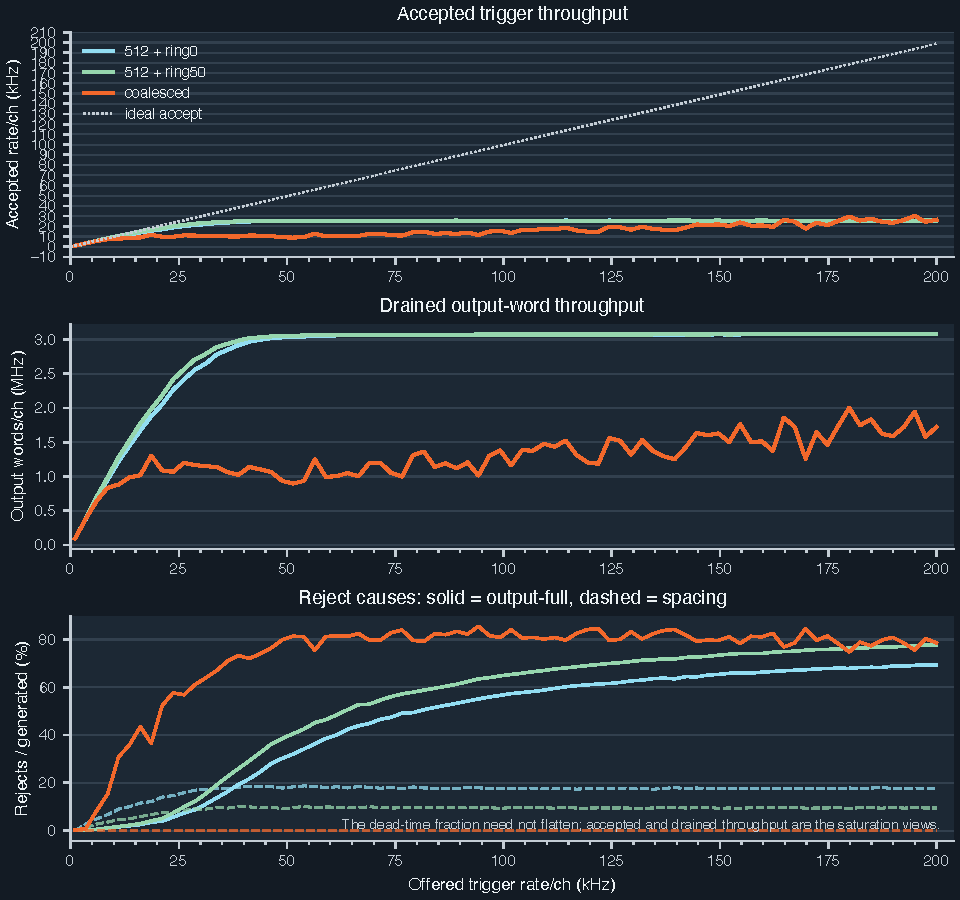
\includegraphics[width=\linewidth,height=0.63\textheight,keepaspectratio]{figures/deadtime_ring_coalesced_throughput.pdf}
\end{frame}

\begin{frame}{Backup: The Fraction Keeps Rising By Definition}
\footnotesize
\[
D(\lambda)=1-\frac{A(\lambda)}{G(\lambda)}
\]

\textbf{Interpretation:}
When accepted throughput \(A(\lambda)\) saturates but generated rate \(G(\lambda)\) keeps increasing, the dead fraction continues to rise. The quantities that flatten are accepted record rate and drained output-word rate.

\vspace{0.8em}
\textbf{Transport scale:}
\[
\frac{\SI{62.5}{\mega\hertz}}{20} \approx \wordshare
\]
For \SI{120}{\word} records, this corresponds to about \throughputceiling.
\end{frame}

\begin{frame}{Backup: Model Validation}
\footnotesize
\begin{columns}[T,onlytextwidth]
\column{0.56\textwidth}
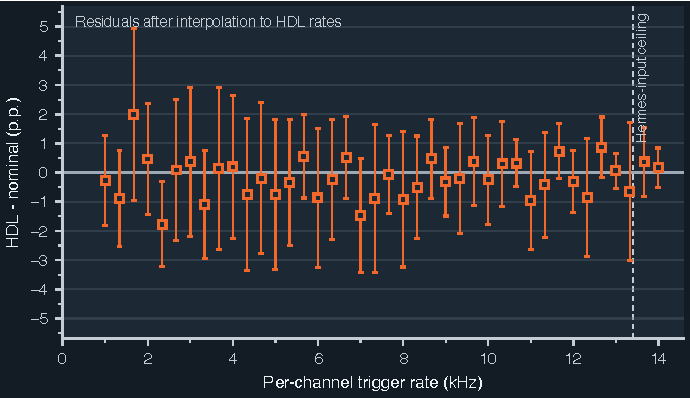
\includegraphics[width=\linewidth,height=0.55\textheight,keepaspectratio]{figures/deadtime_residuals_dunenoir_40pt.pdf}

\column{0.40\textwidth}
\begin{tabular}{@{}lr@{}}
\toprule
Mean absolute residual & \num{0.83} p.p. \\
Maximum absolute residual & \num{2.97} p.p. \\
Mean HDL spread & \num{1.20} p.p. \\
Maximum HDL spread & \num{3.81} p.p. \\
\bottomrule
\end{tabular}

\vspace{0.8em}
The stochastic model is adequate for ranking options. New frame policies still need HDL spot checks.
\end{columns}
\end{frame}

\begin{frame}{Backup: Acceptance Rules I}
\scriptsize
\begin{block}{Legacy}
\[
\mathrm{accept}(i,t) \iff t \ge b_i \wedge \neg\mathrm{progFull}_i(t),
\qquad b_i \leftarrow t+\tau_b.
\]
\end{block}

\begin{block}{Ring}
\[
\mathrm{accept}(i,t) \iff
\mathrm{spacingOK}\wedge\mathrm{queueOK}\wedge\mathrm{ringOK}\wedge
\neg\mathrm{progFull}_i(t).
\]
For \texttt{ring50}, \(\mathrm{spacingOK}\) is a \SI{256}{\sample} same-channel window for a \SI{512}{\sample} record.
\end{block}
\end{frame}

\begin{frame}{Backup: Acceptance Rules II}
\scriptsize
\begin{block}{Coalesced probe}
\[
\mathrm{accept}(i,t) \iff
\mathrm{queueOK}\wedge\mathrm{ringOK}\wedge\neg\mathrm{progFull}_i(t).
\]
Overlapping trigger windows extend or join one queued output interval.
\end{block}
\end{frame}

\begin{frame}{Backup: Data Provenance}
\small
\begin{itemize}
  \item Simulation repo: \texttt{daphne\_mezz\_xc\_sim}, branch \texttt{marroyav/deadtime-tail512-study}, commit \texttt{36073b1}.
  \item Firmware branch for grouped-Hermes RTL: \groupbranch, build commit \groupcommit.
  \item Full-chain RTL CSVs: \texttt{deadtime\_grouped\_hermes\_src5\_ch8\_hdl.csv} and \texttt{deadtime\_grouped\_hermes\_src10\_ch4\_hdl.csv}.
  \item \num{1024} C++ CSVs: \texttt{deadtime\_1024\_...\_cpp.csv}; these are not full-chain RTL because the live source/serializer constants are currently \num{512}.
  \item Latest plots copied from \texttt{data/output/plots} on May 14, 2026: \texttt{deadtime\_grouped\_current\_arch\_compare} and \texttt{deadtime\_1024\_variant\_compare}.
\end{itemize}
\end{frame}

\end{document}
